% This is samplepaper.tex, a sample chapter demonstrating the
% LLNCS macro package for Springer Computer Science proceedings;
% Version 2.20 of 2017/10/04
%
\documentclass[runningheads]{llncs}
%
\usepackage{color}
\usepackage{graphicx}
\usepackage{subfigure}
\usepackage{braket}
\usepackage[final]{fixme}
\usepackage{amsmath,amsfonts}
\usepackage{algorithm}
\usepackage[noend]{algpseudocode}
\usepackage{appendix}

\newcommand{\pp}[2]{\frac{\partial #1}{\partial #2}}
\newcommand{\dede}[2]{\frac{\delta #1}{\delta #2}}
\newcommand{\dd}[2]{\frac{\diff#1}{\diff#2}}
\newcommand{\half}{\frac 12}

\newcommand{\norm}[2]{\| #1 \|_{ #2 }}
\newcommand{\vnorm}[1]{\norm{ #1 }{V}}
\newcommand{\hnorm}[1]{\norm{ #1 }{H}}
\newcommand{\ltwonorm}[1]{\norm{ #1 }{2}}
\newcommand{\diff}[1]{\text{d} #1}

\newcommand{\Q}{\mathbf{q}}
\newcommand{\U}{\mathbf{u}}
\newcommand{\Z}{\mathbf{z}}
\newcommand{\V}{\mathbf{v}}
\newcommand{\Rd}{\mathbb{R}^{d}}
\newcommand{\RdM}{\mathbb{R}^{d\times M}}
\newcommand{\nuinf}{\nu_\text{inf}}

\newtheorem{assumption}{Assumption}

% Used for displaying a sample figure. If possible, figure files should
% be included in EPS format.
%
% If you use the hyperref package, please uncomment the following line
% to display URLs in blue roman font according to Springer's eBook style:
% \renewcommand\UrlFont{\color{blue}\rmfamily}

\begin{document}
%
\title{MCMC for selective metamorphosis with applications to landmarks}
%
%\titlerunning{Abbreviated paper title}
% If the paper title is too long for the running head, you can set
% an abbreviated paper title here
%
\author{Andreas Bock\inst{1} \and  Alexis Arnaudon\inst{1} \and Colin Cotter\inst{1}}
%
\authorrunning{Bock et al.}
% First names are abbreviated in the running head.
% If there are more than two authors, 'et al.' is used.
%
\institute{Imperial College London}
%\email{lncs@springer.com}\\
%\url{http://www.springer.com/gp/computer-science/lncs} \and
%ABC Institute, Rupert-Karls-University Heidelberg, Heidelberg, Germany\\
%\email{\{abc,lncs\}@uni-heidelberg.de}}
%
\maketitle              % typeset the header of the contribution

\begin{abstract}


\keywords{LDDMM \and MCMC \and Metamorphosis.}
\end{abstract}

\section{Introduction}

In computational anatomy
\cite{grenander1994representations,grenander1998computational}, one of the most
fundamental problem is to continuously deform an image, or shape into another
and thereby obtain a natural notion of distance between them, from the energy
required for this deformation.  These distances can then be used for image
registration, atlas construction, etc\dots see \cite{todo} for more
applications. On of the most common method to compute image deformations is
based on the notion of diffeomorphic deformations which assume that the images
are continuously deformed into one another with the additional property that the
inverse deformation is also continuous.  This is a strong requirement for images
which implies that the 'mass' of any part of the image is conserved: we cannot
create or close 'holes'.  This property is also a crucial property of fluid
mechanics, and in fact, the theory of diffeomorphic matching carrying the
moniker \emph{Large Deformation Diffeomorphic Metric Mapping}
\cite{trouve1998diffeomorphisms,beg2005computing} (LDDMM) has been inspired by
fluid mechanics. Indeed, one of the central pillars on which this field relies
is the observation made by Arnold \cite{arnold1966geometrie} that the geodesic
equations for the diffeomorphism group induced by divergence-free vector fields
corresponded to that of incompressible flows. See also ({\color{red} Refs of
Darryl, etc\dots.}{\color{green} Not too sure which fluids papers to reference
here!}) 

If one does not want or need to have a strict diffeomorphic matching, an
extension of LDDMM called metamorphosis
\cite{trouve2005metamorphoses,holm2009euler} is available which introduces a
parameter $\sigma^2$ parametrizing the deviation from diffeomorphic matching.
In particular, if $\sigma^2=0$, metamorphosis reduces to LDDMM.  See
\cite{trouve1995infinite,trouve2005local,miller2001group} for technical details
pertaining to constructing the metamorphosis problem. This theory allows one to
match images of shapes with different topological features, which would have
been near impossible with the standard LDDMM.  Indeed, even for if we allow
inexact matching in LDDMM, the image deformation will have to be close to the
limit of the diffeomorphic matching, yielding a large and uncertain energy for
the matching, thus a useless notion of distance between images.  The incertainty
comes from the fact that for inexact matching, several almost trajectories of
deformations can be computed, but with different energies.  Introducing the
metamorphosis parameter $\sigma^2$ will stabilize this matching problem at the
cost of breaking the diffeomorphic property on the whole image, or shape, and at
all time in the deformation. 

In this work, we modify the original metamorphosis problem to include an image
dependent metamorphosis parameter $\nu(x)$ in order to obtain an almost
diffeomorphic matching, but without the energy or inexact matching problem, see
figure \ref{fig:mm_lddmm}.  If $\nu(x) = \sigma^2$, our theory will reduces to
the standard metamorphosis model, but with a localised $\nu(x)$, we can
selectively introduce metamorphosis on an image and model local topological
effects, such as hole creation or annihilation.  The difficulty of this problem
is to infer the function $\nu(x)$ without a priory knowledge of the location of
the topological effects.  We will use a Markov chain approach to infer good
functions $\nu(x)$, such that the topological effects are well described and a
large part of the matching remains diffeomorphic.  For this paper, we will focus
on landmark matching, but the theory of selective metamorphosis can be extended
to any data structures that the classical metamorphosis of LDDMM theory can
handle, see {\color{red} cite next paper in preparation!}. 


\begin{figure}
\centering
\begin{minipage}{\textwidth}
  \centering
    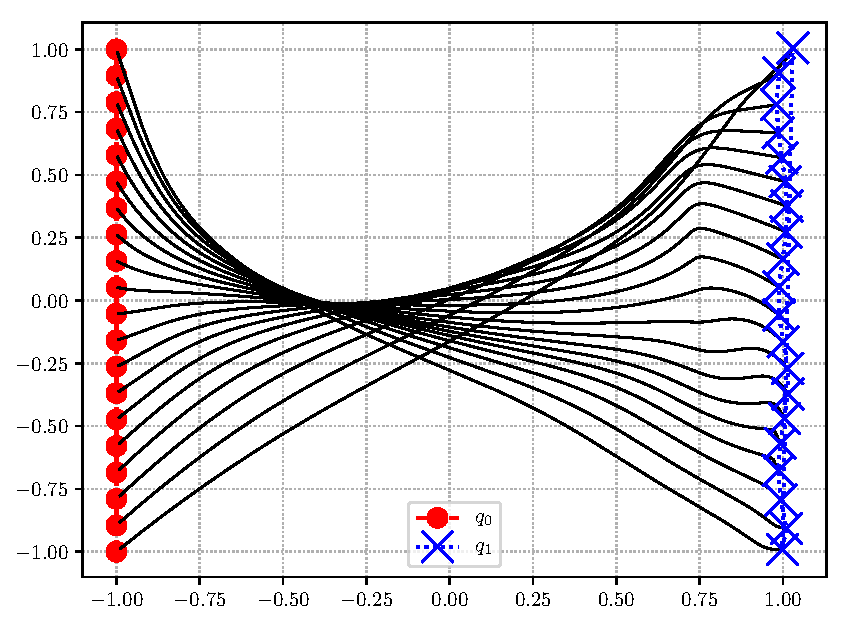
\includegraphics[width=.3\textwidth]{lddmm_criss_cross.pdf}\quad
    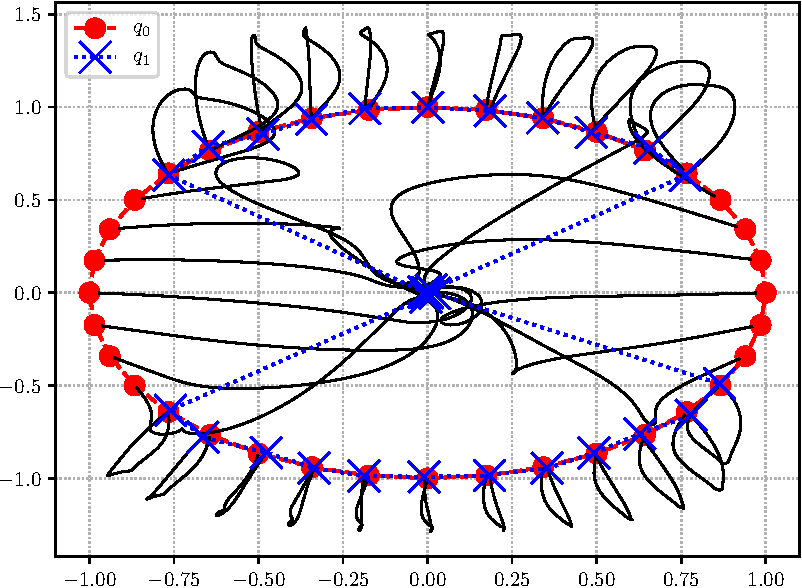
\includegraphics[width=.3\textwidth]{lddmm_squeeze.pdf}\quad
    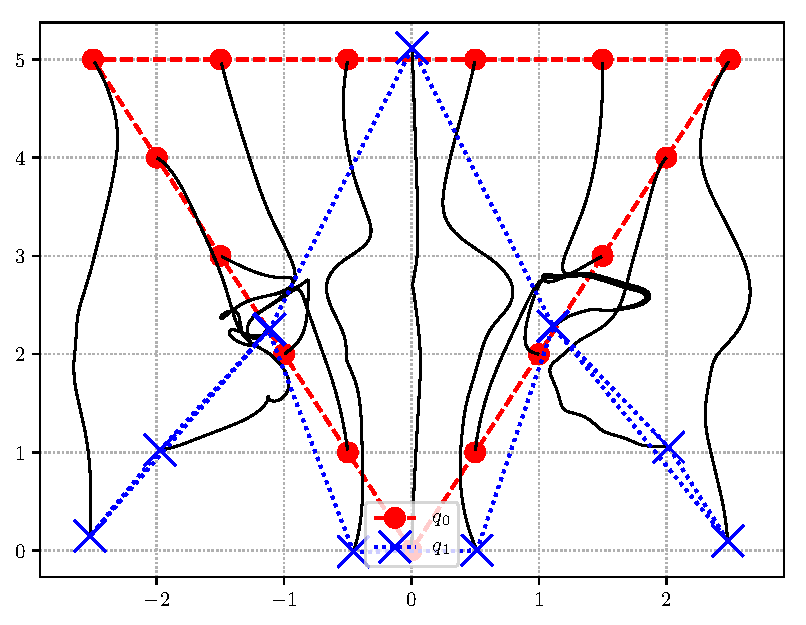
\includegraphics[width=.3\textwidth]{lddmm_triangle_flip.pdf}\\[0.25cm]
    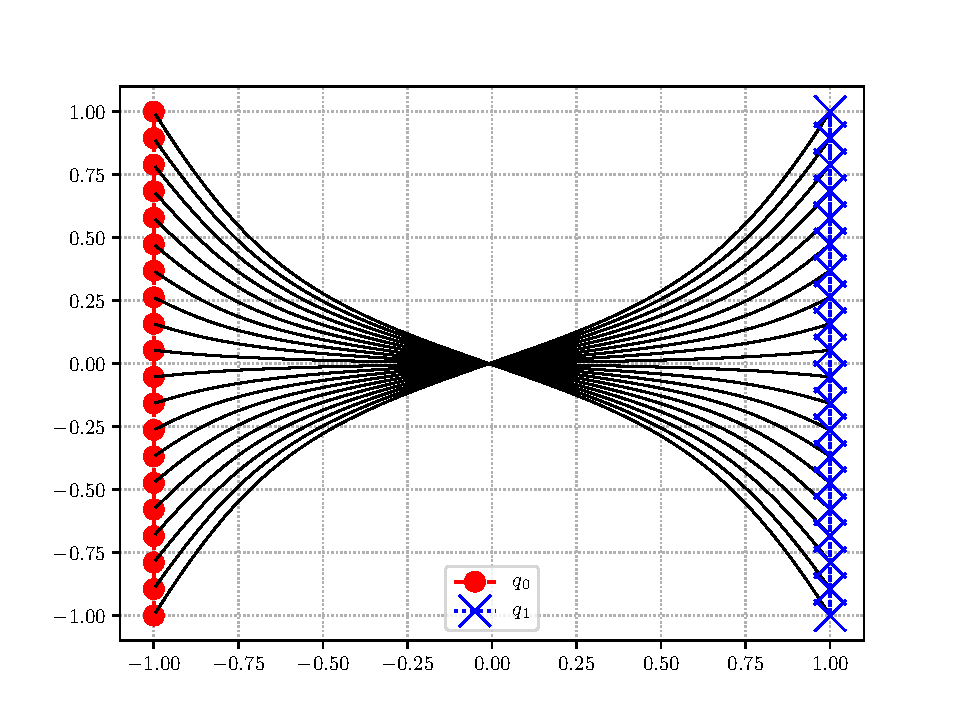
\includegraphics[width=.3\textwidth]{mm_criss_cross.pdf}\quad
    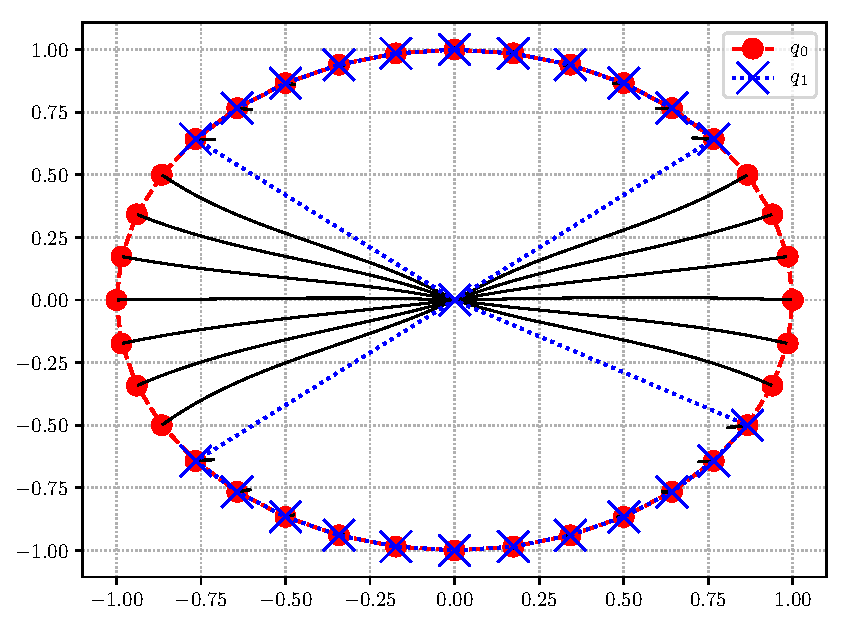
\includegraphics[width=.3\textwidth]{mm_squeeze.pdf}\quad
    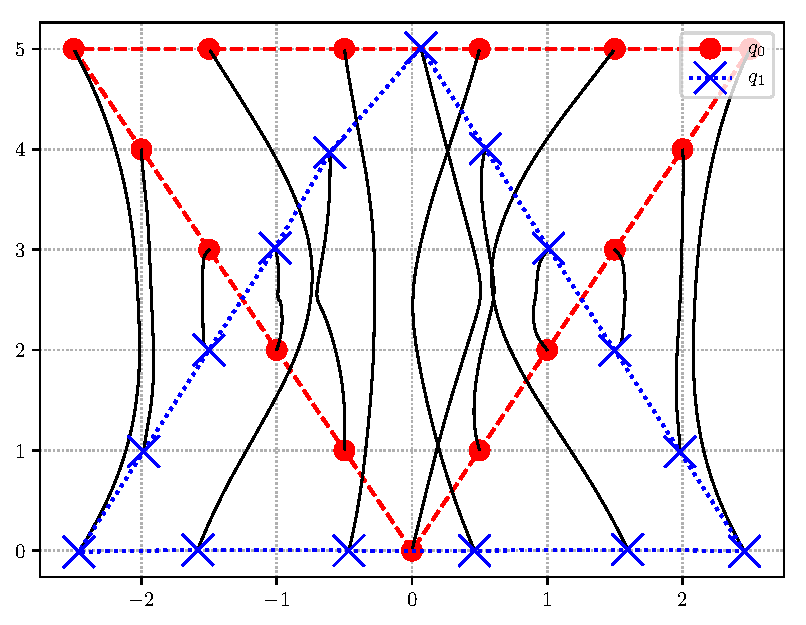
\includegraphics[width=.3\textwidth]{mm_triangle_flip.pdf}\\[0.25cm]
    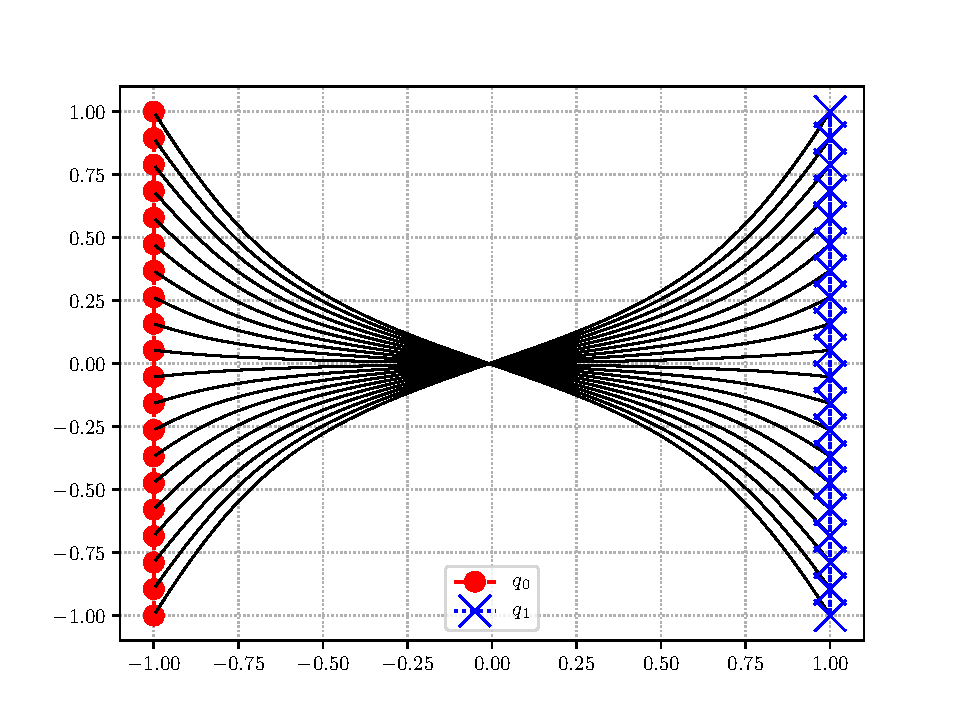
\includegraphics[width=.3\textwidth]{mm_criss_cross.pdf}\quad
    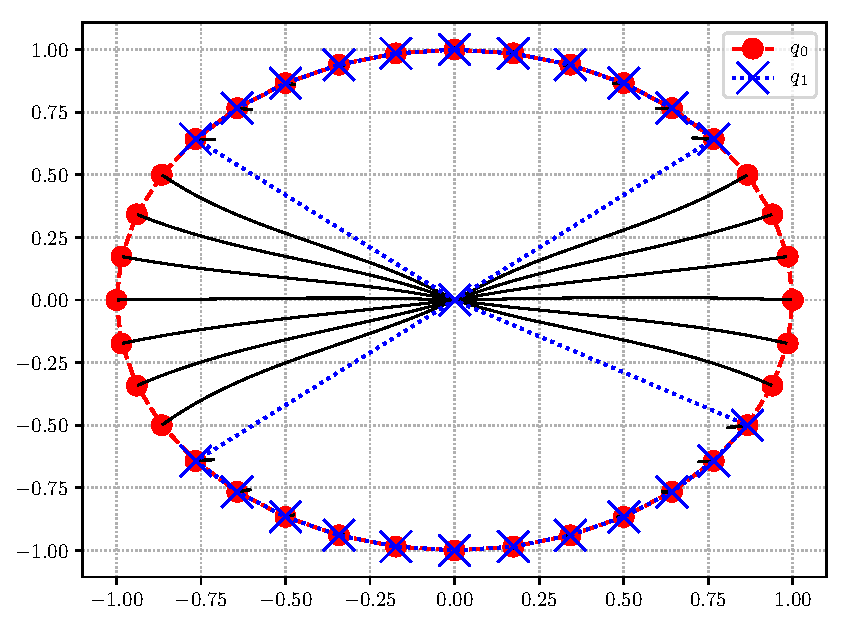
\includegraphics[width=.3\textwidth]{mm_squeeze.pdf}\quad
    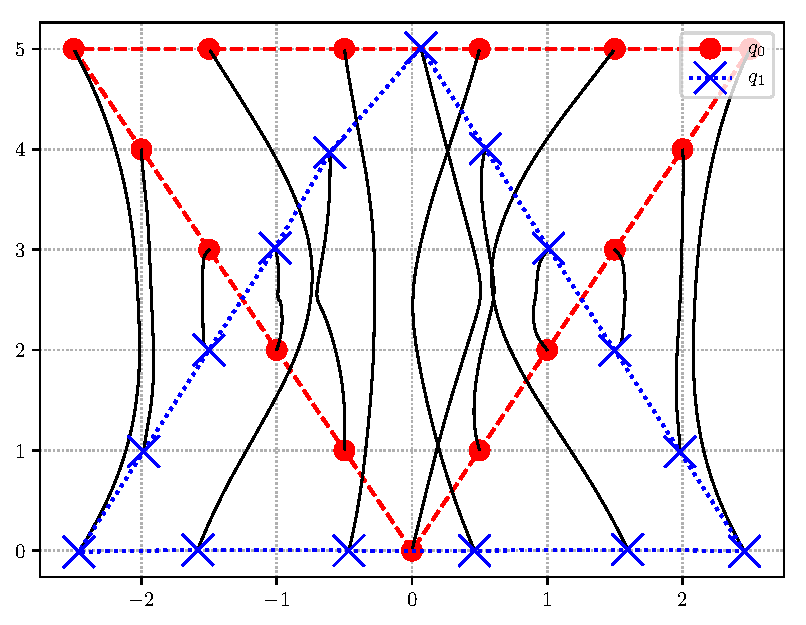
\includegraphics[width=.3\textwidth]{mm_triangle_flip.pdf}
    \caption{This figures illustrates landmark matching with classical LDDMM
    (top row), metamorphosis (bottom row) and selective metamorphosis (middle
    row).  We chose difficult matching for LDDMM, and we observe unrealistic
    landmark trajectories, with large resulting energies, or distances, whereas
    the metamorphosis  matching results in a more realistic landmark
    trajectories.  The selective metamorphosis has the extra advantage of only
    breaking the diffeomorphic property where needed in along the matching, thus
    preserving more of the desired diffeomorphic property of the matching.
    {\color{red} Add the middle row with position of $\nu$ fields as crosses,
    and value of the energy functional for each (larger for top and middle
    row)}}
    \label{fig:mm_lddmm}
\end{minipage}
\end{figure}

%In this paper we consider a generalisation of the classical metamorphosis
%problem. The purpose of this work is to allow singular control where
%metamorphosis occurs in space to allow practitioners in e.g. medical imaging to
%qualitatively assess different growth patterns. Owing to this observation we
%build a stochastic model on spatial domain and use develop an MCMC algorithm in
%order to infer where in space growth is the most likely.\\

{\bf Structure} This paper is organised as follows. We review the theory of
classical metamorphosis in section \ref{sec:bg} and extend it to selective
metamorphosis in \ref{sec:select_mm}.  We then introduce a Bayesian framework
for inferring the local metamorphosis parameter $\nu(x)$ in section
\ref{sec:bayesian} and apply this theory to a few landmark examples in section
\ref{sec:numerical}.

\section{Metamorphosis with landmarks}\label{sec:bg}

In this paper we are concerned with diffeomorphometric approaches to image and
shape matching. One of the central pillars on which this field relies is the
observation made by Arnold \cite{arnold1966geometrie} that, under certain
conditions, a time-dependent velocity field $u$ e.g. occupying some Hilbert
space $u_t \in V$ induces a curve on a subgroup $G_V$ of diffeomorphisms
\cite{younes2010shapes} via the following ordinary differential equation
\begin{align}
& \dot{\varphi_t} = u_t \circ \varphi_t\, , \qquad  \varphi_0 = \text{id}
  \label{diffeo}
\end{align}
with $\varphi_t \in G_V$, $\forall t$ and $u_t$ is a time-dependent vector
field, obtained as a solution of the optimisation problem
\begin{align}
  E(u_t) = \min_{\hat u_t} \int_0^1 \half\vnorm{\hat u_t}^2 \diff{t} +
  \frac{1}{\sigma^2} S(I_0\circ\varphi_1, I_1)\, , \label{E-def}
\end{align}
where $S$ denotes a similarity measure or norm between the deformed initial
image $I_0\circ \varphi_1$ and the target image $I_1$ to allow inexact matching
parametrised by $\sigma^2$. The LDDMM) approach takes $S$ as an $L^2$ norm on the difference between
its arguments.
In the sequel, we will set $\lambda=0$ such that we
only consider exact matching, the hardest problem to solve, especially for
images non-topologically equivalent, as discussed in the introduction, see also
Fig. \ref{fig:mm_lddmm}.

In order to simplify the exposition, we will consider singular solutions of this
problem, which are given by \begin{align}
  \frac{\delta l}{\delta u} = m(x) = \sum_i p_i \delta(x-q_i)\,, 
\end{align}
for $N$ landmarks with position $q_i\in \mathbb R^2 $ and momenta $p_i \in \mathbb R^2$. 
The vector field is thus 
\begin{align}
  u(x) = \sum_i p_i K(x-q_i)\,, 
  \label{u-def}
\end{align}
where $K:\mathbb R^2\times \mathbb R^2\to \mathbb R$ is the kernel associated to
the norm $\|\cdot \|_V$.  For metamorphosis, we introduce a discrete template
variable $\boldsymbol \eta_t$ such that the deformation of a set of landmarks is
\begin{align}
  \mathbf q_t = \varphi_t \boldsymbol \eta_t\, . 
  \label{q_t}
\end{align}
Then, we can define the template velocity as 
\begin{align}
  \mathbf z = \varphi_t \dot {\boldsymbol \eta}
  \label{z_eta}
\end{align}
and extend the energy \eqref{E-def} to 
\begin{align}
  \begin{split}
    E_m(u_t,\mathbf z) =\min_{\hat u_t, \hat{\mathbf z}} & \int_0^1
    \half  \left (\vnorm{\hat u_t}^2 + \frac{1}{\sigma^2} \sum_i |\hat{z_i}|^2\right )\diff{t}
  \end{split}
  \label{E_m-def}
\end{align}
where now the reconstruction relation is 
\begin{align}
    \dot{\mathbf q_t} = u_t (\mathbf q_t) + \mathbf z_t\, , 
    \label{dq-m}
\end{align}
obtained from the definition of $z$ and $u$, see \cite{holm2009euler}.  before,
the boundary conditions are given on the positions $\mathbf q(0)$ and $\mathbf
q(1)$, but we now have an extra term in the energy and the reconstruction
equation \eqref{dq-m}. 

By taking variations carefully, see again \cite{holm2009euler}, we directly obtain 
\begin{align}
  m(x) = \frac{1}{\sigma^2} \sum_i z_i\delta(x-q_i)\qquad \Rightarrow \qquad
  z_i = \sigma^2 p_i\, , 
\end{align}
and the equation of motions are
\begin{align}
  \begin{split}
  \dot{\mathbf p_t} &= - \nabla u_t(\mathbf q_t)^T \mathbf p_t\\ 
  \dot{\mathbf q_t} &= u_t(\mathbf q_t) +  \sigma^2\mathbf p_t \,,
  \end{split}
  \label{eq-m-classic}
\end{align}
where $u_t$ is defined in \eqref{u-def}. 

\section{Selective Metamorphosis for Landmarks}\label{sec:select_mm}

We can now extend the metamorphosis setting to be able to locally control the
amount of non-diffeomorphic evolution.  For this, we introduce a positive smooth
bounded function $\nu: \mathbb R^2\to \mathbb R$, with $\mathrm{max}(\nu) =
\nu_m$ which will replace the parameter $\sigma^2$ such that if
$\nu(x)=\sigma^2$, we will recover the classic landmark metamorphosis.  We thus
choose the energy functional to be

We can now extend the metamorphosis setting to be able to locally control the
amount of non-diffeomorphic evolution.  For this, we introduce a function $\nu:
\mathbb R^2\to \mathbb R$ replacing the parameter $\sigma^2$ such that if
$\nu(x)=\sigma^2$, we will recover the classic landmark metamorphosis.
We thus choose the energy functional to be
\begin{align}
  \begin{split}
    E_{sm}(u_t,\mathbf z) =\min_{\hat u_t, \hat{\mathbf z}} & \int_0^1
    \half  \left (\vnorm{\hat u_t}^2 +\sum_i \frac{1}{\nu(q_i)} |\hat{z_i}|^2\right )\diff{t}
  \end{split}
  \label{E_sm-def}
\end{align}

subject to the reconstruction equation \eqref{dq-m}. We have, as before that
\begin{align}\label{zp_relation}
  m(x) =  \sum_i \frac{1}{\nu(q_i)} z_i\delta(x-q_i)\qquad \Rightarrow \qquad
  z_i = \nu(q_i) p_i\, , 
\end{align}

We show that the optimisation problem \eqref{E_sm-def} is well-posed. First, we
have
\begin{assumption}\label{assumption:nu_bounded}
$\mathrm{max}(\nu) = \nu_m < \infty$ and $\nu$ is bounded from below
away from zero by $\nuinf \in \mathbb R$.
\end{assumption}

\begin{theorem}\label{sm-eu}
Assumption \ref{assumption:nu_bounded} implies that the problem
\eqref{pbl:reformulation} attains its unique infimum.\\

Proof: See appendix \ref{app:proof:sm-eu}.
{\hfill $\square$}
\end{theorem}


The problem defined by \eqref{E_sm-def} yields the following equations for
selective metarmorphosis for landmarks:
\begin{align}
  \begin{split}
  \dot{\mathbf p}_t &= - \nabla u_t(\mathbf q_t)^T \mathbf p_t - \sum_i \frac12
  \nabla \nu(q_i) |p_i|^2\\ \dot{\mathbf q}_t &= u_t(\mathbf q_t) +
  \nu(q_i)\mathbf p_t \,.
\end{split}
  \label{eq-m-classic}
\end{align}
Note that via relation \eqref{zp_relation}, if $\nu(x)=0$ in parts of the domain
these equations allow the diffeomorphism to attain non-zero momentum without
moving the image. The equation for the variable $\mathbf z_t$ can be written as 
\begin{align}
  \dot  z_i &= \nabla_i u(\mathbf q_t) z_i\,, 
\end{align}
{\color{blue} indeed, the complete equation is 
\begin{align}
  \frac{d}{dt} \left ( \frac{z}{\nu(q)}\right) = \nabla \left ( \frac{z}{\nu(q)}
  u(q)\right ) - \frac{\nabla \nu(q)}{\nu^2(q)}z^2\, .
\end{align}
}
Notice that these equations are Hamiltons equation for the Hamiltonian, or
energy density function written in term of $\mathbf p_t$ and $\mathbf q_t$
\begin{align}
  h(\mathbf q, \mathbf p) =  \frac12 \sum_{i,j}K(q_i-q_j)p_i\cdot p_j+ \frac12
\sum_i \nu(q_i) |p_i|^2\,.  \end{align}

The goal of this work is to infer the unknown function $\nu$ so as to gather
information about where in the spatial domain we are most likely to observe
metamorphic behaviour via a Bayesian framework as in \cite{dashti2017bayesian}.

Using the equation for $z$, we can write $z_t = z_t \circ \varphi^{-1}$, and
together with the relations \eqref{q_t} and \eqref{z_eta}, we can write
\begin{align*}
  \mathbf q_t &= \varphi_t \mathbf q_0 + \varphi_t \eta_t\\
   &= \varphi_t \mathbf q_0 + \varphi_t \int \dot \eta_t dt\\
   &= \varphi_t \mathbf q_0 + \varphi_t \int \varphi_t^{-1} \varphi_t\dot \eta_t dt\\
   &= \varphi_t \mathbf q_0 + \varphi_t \int  \varphi_t^{-1}\mathbf z dt \\
   &= \varphi_t \mathbf q_0 + \varphi_t \int  \varphi_t^{-1}\nu(\mathbf q_t) \mathbf p_t  dt\\
   &= \varphi_t \mathbf q_0 + \varphi_t \int  \varphi_t^{-1}\mathbf z_0\circ \varphi_t^{-1} dt\, , 
\end{align*}
and directly verify that it satisfy the equation of motions by computing
\begin{align*}
  \dot {\mathbf q}_t = \dot \varphi_t \varphi_t^{-1} \varphi \mathbf q_0 + \dot
  \varphi_t \varphi_t^{-1} \varphi_t \eta_t + \varphi_t \dot \eta_t  = u_t(
  \mathbf q_t) + \mathbf z_t\, ,
\end{align*}
using $\dot \varphi_t\varphi_t^{-1} = u_t$. 
This is the integral form of the equation of motion, which is the same equation
as in \cite{holm2009euler}[eqn 19], thus the same existence and uniqueness
results hold for both the initial value and the boundary value problems.
{\color{red} I AM HERE}

\section{Bayesian Framework}\label{sec:bayesian}

We now place a stochastic model on $\nu$, the purpose of which depends on its
definition as mentioned in remark \eqref{remark:nu}. The goal is to develop an
algorithm to infer $\nu$, passing via the deterministic problem seen above.\\

First we present some preliminaries on the Bayesian approach to inverse problems
in section \ref{subs:gf}, essentially quoting results from
\cite{dashti2017bayesian}.  See also \cite{cotter2013mcmc} for an exposition of
algorithmic aspects of function space MCMC. Section \ref{subs:finite-dim-param}
then describes how we apply this stochastic approach to inverse problems to
$\nu$ by a finite-dimensional family of parameterisations.

\subsection{General Framework}\label{subs:gf}
% General setting
Our setting is the following. Given an inverse problem

$\min\quad J$\\

we formally define a centered Gaussian distribution, denoted $N(0, B)$ over this
space of functions defined up to a constant by the density
\begin{align}
\mu_0 = e^{-J}
\end{align}
In general, for inverse problems on function space, several key properties
documented in \cite{?} must be verified before the inverse-problem is
well-posed. Beyond showing existence of the MAP estimator extremising $J$ above,
the infinite-dimensional version of Bayes' rule must also be check i.e. the
Radon-Nikodym derivative of the prior with respect to the posterior must exist
and be absolutely continuous. Finally, we request continuity of the posterior
distribution w.r.t the initial data corresponding in a sense to Hadamard
well-posedness in a stochastic framework. Proceeding bona fide we therefore have
the key ingredients necessary to define a pCN MCMC algorithm:
\begin{enumerate}
\item Sample a function.
\item $f^{k+1} = \alpha f^k + (1-\alpha) f^k$
\item accept/reject..
\end{enumerate}

\textbf{$\longrightarrow$ Finish}\\

% Talk about our problem
\subsection{Finite-dimensional Parameterisation}\label{subs:finite-dim-param}

We now introduce the main problem of this paper in the setting above. We
consider $\nu$ as a random variable, indeed a random \emph{function}, occupying
some space yet to be determined. This is an appropriate framework because if the
lack of uniqueness allows for a qualitative evaluation of a solution to
selective metamorphosis. In this paper we consider the case where $\nu$ is given
by a sum of exponentials:
\begin{equation}
    \nu_h (x) := \sum_k e^{-\|h_k - x\|_{\Rd}^2}
\end{equation}
Here the finite family $h_k$ of centroids in $\Rd$ fully determine $\nu_h$, thus
greatly reducing the complexity of sampling.

\begin{align}
	\Phi(a_k) = S(\nu,q_0,q_1) + |\nu|_V^2
\end{align}
where, for example $ V = {L_2(\mathcal D)}$.

\newcommand{\mhsample}{\textsc{sampleCentroid}}
\newcommand{\acceptprob}{\textsc{acceptanceProbability}}

\begin{algorithm}[h!]
\begin{algorithmic}
\caption{MCMC on $\nu$}\label{algo:mcmc}
\Procedure{quasiMCMC}{$N$}
\State $k \gets 0$
\State $\nu^k \gets \text{ some initial guess}$
\While{$k < N$}
\State $\nu \gets \mhsample ()$\hspace{3cm} \textbf{\# sample a new centroid}
\State $(q, z, u) \gets $
\If {\textsc{randomUnit()}$\,< \acceptprob(q, z)$}
    \State do update
\Else
    \State don't do update
\EndIf
\State $k\gets k+1$
\EndWhile
\Return $q^k,\, z^k,\, u^k$
\EndProcedure
\end{algorithmic}
\end{algorithm}

Note that the $solveMetamorphosis()$ operation, in general, depends on how the
spatial domain is treated e.g. whether we use landmarks or treat full images.
In this paper we are only concerned with the former, so we use a standard and
easily implemented procedure (cite) below 

\textbf{$\longrightarrow$ Describe shooting/solution method}\\
\begin{algorithm}[h!]
\begin{algorithmic}
\caption{Metamorphosis for fixed $\nu$}
\Procedure{solveMetamorphosis}{}
\State something either shooting or Firedrake
\EndProcedure
\end{algorithmic}
\end{algorithm}

\textbf{$\longrightarrow$ Something about adjoints here}\\

\section{Numerical examples}\label{sec:numerical}

This penultimate section displays some numerical results for our method. First,
as a proof of concept 
%Stuff that works:
%\begin{tabular}{ l c r }
%\text{Test case}   & \beta \text{ (pCN) } & \text{Samples} \\
%\text{Criss-cross} & & \\ <-- CENTROID
%\text{Triangle}    & & \\
%\text{Pringle}     & & \\
%\text{Squeeze}     & 1 & 500 <-- CENTROID
%\end{tabular}

As we have seen in figure \ref{fig:mm_lddmm}, classic metamorphosis is an
appropriate model for non-diffeomorphic matching. We now evaluate our stochastic
model described in algorithm \ref{algo:mcmc} to the landmark configurations in
\ref{fig:mm_lddmm}.

\begin{figure}
\centering
\begin{minipage}{\textwidth}
  \centering
    \includegraphics[width=.2\textwidth]{example-image-a}\quad
    \includegraphics[width=.2\textwidth]{example-image-a}\quad
    \includegraphics[width=.2\textwidth]{example-image-a}\quad
    \includegraphics[width=.2\textwidth]{example-image-a}\\[0.25cm]
    \includegraphics[width=.2\textwidth]{example-image-a}\quad
    \includegraphics[width=.2\textwidth]{example-image-a}\quad
    \includegraphics[width=.2\textwidth]{example-image-a}\quad
    \includegraphics[width=.2\textwidth]{example-image-a}
    %\subcaption{.}
    \caption{Selective metamorphosis for the inverted landmarks example The top
    row displays the geodesics corresponding a sample realisation from the
    chain, centroid heat map with four MAP estimators, functional histogram and
    autocorrelation plot. The bottom row shows the geodesics for four MAP
    estimators.}
    \label{fig:selective:crisscross}
\end{minipage}
\end{figure}
\begin{figure}
\centering
\begin{minipage}{\textwidth}
  \centering
    \includegraphics[width=.2\textwidth]{example-image-a}\quad
    \includegraphics[width=.2\textwidth]{example-image-a}\quad
    \includegraphics[width=.2\textwidth]{example-image-a}\quad
    \includegraphics[width=.2\textwidth]{example-image-a}\\[0.25cm]
    \includegraphics[width=.2\textwidth]{example-image-a}\quad
    \includegraphics[width=.2\textwidth]{example-image-a}\quad
    \includegraphics[width=.2\textwidth]{example-image-a}\quad
    \includegraphics[width=.2\textwidth]{example-image-a}
    %\subcaption{.}
    \caption{Selective metamorphosis for the pinch example. The top row displays
    the geodesics corresponding a sample realisation from the chain, centroid
    heat map with four MAP estimators, functional histogram and autocorrelation
    plot. The bottom row shows the geodesics for four MAP estimators.}
    \label{fig:selective:pinch}
\end{minipage}
\end{figure}

\textbf{$\longrightarrow$ Explain results}\\

\begin{figure}
\centering
\begin{minipage}{\textwidth}
  \centering
    \includegraphics[width=.2\textwidth]{example-image-a}\quad
    \includegraphics[width=.2\textwidth]{example-image-a}\quad
    \includegraphics[width=.2\textwidth]{example-image-a}\quad
    \includegraphics[width=.2\textwidth]{example-image-a}\\[0.25cm]
    \includegraphics[width=.2\textwidth]{example-image-a}\quad
    \includegraphics[width=.2\textwidth]{example-image-a}\quad
    \includegraphics[width=.2\textwidth]{example-image-a}\quad
    \includegraphics[width=.2\textwidth]{example-image-a}
    %\subcaption{.}
    \caption{Selective metamorphosis for the inverted landmarks example. The top
    row displays the geodesics corresponding a sample realisation from the
    chain, centroid heat map with four MAP estimators, functional histogram and
    autocorrelation plot. The bottom row shows the geodesics for four MAP
    estimators.}
    \label{fig:selective:triangle}
\end{minipage}
\end{figure}

% Insert Effective Sample size (if time)
We note that since the Euler-Lagrange equations for $p$ and $q$ are
time-reversible, the configuration in both lead to a notion of
collapse and hole creation for the landmarks.\\



We note that the source code for all of these experiments is documented
here (insert link to github.io). 

\section{Outlook}\label{sec:outlook}

{\color{red} Nice sentence:} {\color{blue} This could provide a
first-order exploratory tool for physicians, to see if the development of a
biological feature stems from a few violations of diffeomorphic evolution.}


Another choice is 
\begin{align}
    l(q,p) = \|u\|_B^2 + \sum_i p_i\cdot \nu(q_i) \, , 
\end{align}
where $\nu:\mathbb R^2 \to \mathbb R^2$, which will give more freedom on the
metamorphosis term, and give equations of motion as \begin{align}
    \dot p_i  &= \nabla u(q_i)p_i  + p_i \cdot \nabla \nu(q_i)\\
    \dot q &= u(q_i) + \nu(q_i) 
\end{align}

Natural extensions of this work include fully determining e.g. the Fourier modes
of $\nu$ via the stochastic framework.\\

Future work also includes extending this framework to images e.g. using the
kernel framework in \cite{richardson2016metamorphosis}, or developing a
space-time method. Formalising the measure-theory necessary to consider the
limit of ? as $k\rightarrow\infty$.\\

Moreover, adding a time-dependency to $\nu$ is also to be explored. It is our
hope that we can extend the theory developed here to encompass classic
metamorphosis; that is to say, to develop the necessary theory in order to place
a stochastic model on the state space consisting of velocities and source
functions. Being able to sample random pairs (MCMC) of these would permit a
novel numerical approach to metamorphosis as well as other problems shape
analysis.

\appendix

\section{Proof of Theorem \ref{sm-eu}}\label{app:proof:sm-eu}
In this section we analyse the problem described in \eqref{pbl:selective_mm} for
an a priori known function $\nu$ which we denote \emph{selective metamorphosis
problem}. The first task is to show that the functional attains its infimum,
i.e. identification of a minimiser. We begin with the following assumption:


Since the limit as $\nu\rightarrow 0$ is well-understood these assumptions do
not constitute large concessions. Clearly the functional in \eqref{nu_fnl} is
not convex, so we work with a reformulation to ensure the required weak lower
semi-continuity. This comes at the cost of showing weak continuity of the
constraint variables. Specifically, we define a variable $z^i_t = p^i_t
\sqrt{\nu(q_t^i)}$ in the problem:
\begin{align}
\inf_{\substack{u \in L^2([0,1],V)\\ q, z\, \in L^2([0,1],\RdM)}}
    & S = \int_0^1 \half\vnorm{u_t}^2 + \half\sum_i |z_t^i|^2 \diff{t}\\
    & \dot{q_t^i} = u(q_t^i) + \sqrt{\nu(q_t^i)} z^i_t\\
    & q_0,\,q_1\text{ fixed}
  \label{pbl:reformulation}
\end{align}

We now show existence of a minimiser to this problem. First, note that owing to
the constraint effectively being a boundary value problem, we cannot always find
a $q$ for arbitrary pairs of $(u,\,z)$. We define an bounded operator
$(q,u)\mapsto frac{\dot{q} - u(q)}{\sqrt{\nu(q)}} := z$:
\begin{align*}
\ltwonorm{z}^2 & = \ltwonorm{\frac{\dot{q} - u(q)}{\sqrt{\nu(q)}}}^2\\
& \leq \nuinf^{-1}\Big(\ltwonorm{\dot{q}}^2 + \ltwonorm{u(q)}^2\Big)\\
\end{align*}
which is clearly bounded since $q\in C^1(0,1,H)$ and since by continuity of $u$.
From this we generate a minimising sequence $(q^n, u^n, z^n)$ admissible to
\eqref{pbl:reformulation}.\\

\textbf{$\longrightarrow$ Show weak continuity of the constraint equation for
$q$ (the stuff below)}\\

Passing to subsequences where necessary we can by classic results
\cite{younes2010shapes} extract bounded subsequences converging to weak limits
where necessary. By convexity of $S$ we have therefore proved the following:

\begin{theorem}
Assumption \ref{assumption:nu_bounded} implies that the problem
\eqref{pbl:reformulation} attains its unique infimum.
{\hfill $\square$}
\end{theorem}

We now derive the optimality conditions of \eqref{pbl:reformulation}.
Using $p_t^i$ as a Lagrange multiplier and extremising $J$ leads to the
following equations:

%\begin{subequations}
\begin{align}
& \dot{p_t^i} + \nabla u(q_t^i) p_t^i + \half \nabla \nu(q_t^i) |p_t^i|^2 = 0\\
& \dot{q_t^i} = u(q_t^i) + \nu(q_t^i) p^i_t\\
& q_0,\,q_1\text{ fixed}
\end{align}
  \label{pbm:nonlinear_inner:optimality}
%\end{subequations}

In this paper we are concerned only with
landmarks, so we can write the Lagrangian in terms of the state variables $\hat
l(q, z) = \hat l(u, q, z)$ \cite{younes2010shapes}:
\begin{align*}
\vnorm{u}^2 = \sum_{i,j=0}^M K(q^i,q^j) p^i \cdot p^j
\end{align*}

where supercripts denote the landmark index. 
%\inf_{\substack{u \in L^2([0,1],V)\\ q, z\, \in L^2([0,1],\RdM)}}
    %& S = \int_0^1\sum_{i,j=0}^M K(q_t^i,q_t^j)
  %& \dot{q_t^i} = \sum_{j=0}^M K(q_t^j, q_t^i)p_t^i + \sqrt{\nu(q_t^i)} z^i_t\\

Extremising the action $S$ we obtain the equations: 
\begin{align}\label{pq:optimality}
& \dot p_i =\frac12 \sum_j \nabla K(q_i,q_j)p_i\cdot p_j  + \frac12 |p_i|^2
\nabla \nu(q_i)\\
& \dot q_i = \sum_j K(q_i,q_j)p_i + \nu(q_i)p_i\\
& q_0,\,q_1\text{ fixed}
\end{align}

\begin{theorem}[Optimality Conditions]
There exists a unique (? )solution $u, q, z$ to this system.

This will give more conditions on $\nu$, like $\nu(x) \in C^{1}(\mathbb R^2)$. 
\end{theorem}

\bibliographystyle{abbrv}
\bibliography{landmarks}




\end{document}

